
\documentclass[twoside,a4paper]{refart}

\usepackage[utf8]{inputenc}
\usepackage[T1]{fontenc}
\usepackage[english]{babel}

\usepackage{makeidx}
\usepackage{ifthen}

\usepackage[toc,page]{appendix}

\usepackage{graphicx}
\usepackage{xcolor}

\usepackage{hyperref}

\usepackage{mathtools}
\usepackage{amsmath}
\usepackage{amssymb}
\usepackage{upgreek}

\usepackage{subfloat}
\usepackage{subfig}

\usepackage{tabularx}
\usepackage{multicol}
\usepackage{multirow}
\usepackage{booktabs}

\usepackage[english]{varioref}

% new commands
\newcommand{\asf}{ASF\texttt{++}~}
\newcommand{\omnet}{OMNeT\texttt{++}~}
\newcommand{\mail}[1]{\textcolor{red!70!black}{\href{mailto:#1}{\texttt{#1}}}}
\newcommand{\ie}{i.\,e.,}
\newcommand{\eg}{e.\,g..}

 % backslash in \tt font.
\def\bs{\char'134 }

\DeclareRobustCommand\cs[1]{\texttt{\char`\\#1}}

% declare math operators
\DeclareMathOperator{\avg}{avg}
\DeclareMathOperator{\abs}{abs}
\DeclareMathOperator{\fix}{fix}
\DeclareMathOperator{\rnd}{rnd}
\DeclareMathOperator{\lin}{lin}
\DeclareMathOperator{\mymed}{med}
\DeclareMathOperator{\mysgn}{sgn}
\DeclareMathOperator{\mysqr}{sqr}
\DeclareMathOperator{\mytri}{tri}
\DeclareMathOperator{\mysaw}{saw}
\DeclareMathOperator{\mysym}{sym}
\DeclareMathOperator{\myshp}{shp}
\DeclarePairedDelimiter\floor{\lfloor}{\rfloor}
\usepackage[utf8]{inputenc}
\usepackage[T1]{fontenc}
\usepackage[english]{babel}

\usepackage{listings}
\usepackage{xcolor}

% define color
\definecolor{commentgreen}{rgb}{.133,.545,.133}
\newcommand{\bash}{\color[rgb]{0.0,0.35,0.7}}

% listing settings
\lstset{	
	columns=flexible,
	basicstyle=\ttfamily,
	frame=single,
	breaklines=true,
	basicstyle=\footnotesize,
	showstringspaces=false,
	tabsize=2,
	%upquote=true,
}

\lstdefinelanguage{terminal}{
	basicstyle = \footnotesize\ttfamily,
	literate={~} {{$\sim$}}1 {-} {{-}}1 {*} {{*}}1 {+} {{\texttt{+}}}1 {_} {{\texttt{\_}}}1 {=} {{\texttt{=}}}1,
	moredelim=[is][\bash]{@}{@},
}

\lstdefinelanguage{ned}{
	basicstyle = \footnotesize\ttfamily,
	morestring=[s][\color{violet!90!black}]{"}{"},
	morecomment=[l][\color{commentgreen}]{//},
	keywordstyle=\color{blue!80!black},
	morekeywords={package, import, network, simple, gates, parameters, submodules, connections, allowunconnected, string, double, int, char, datarate, default, for, if, like, module}
}

\lstdefinelanguage{xml}{
	morestring=[b]",
	morecomment=[s]{<?}{?>},
	morecomment=[s][\color{orange!85!black}]{<!--}{-->},
	basicstyle = \footnotesize\ttfamily,
	stringstyle=\color{black},
	identifierstyle=\color{blue!60!red},
	keywordstyle=\color{blue!60!red},
	morekeywords={FamilyTree,ScroogeMcDuck,HortenseMcDuck,DonaldDuck}
	morekeywords={configuration, Physical, Conditional, Unconditional, start_time, node, action, filter, var, frequency, name, parameters},
}

\lstdefinelanguage{ini}{
	morestring=[s][\color{violet!90!black}]{"}{"},
	morestring=[s][\color{red!70!black}]{[}{]},
	morecomment=[l][\color{commentgreen}]{//},
	basicstyle = \footnotesize\ttfamily,
	keywordstyle=\color{blue!90!black}\ttfamily,
	stringstyle=\color{red!70!blue}\ttfamily,
	commentstyle=\color{commentgreen}\ttfamily,
	numberstyle=\tiny,
	morekeywords={network, {sim-time-limit}},
	moredelim=[is][\color{blue!90!black}]{@}{@}
}

\lstdefinelanguage{cpp}{
	language=C++,
	numbers=left,
	morestring=[s]{"}{"},
	basicstyle = \scriptsize\ttfamily,
	keywordstyle=\color{blue!90!black}\ttfamily,
	stringstyle=\color{red!70!blue}\ttfamily,
	commentstyle=\color{commentgreen}\ttfamily,
	numberstyle=\tiny,
	morekeywords={}
}

\lstdefinelanguage{adl}{
	basicstyle = \footnotesize\ttfamily,
	commentstyle=\color{commentgreen}\ttfamily,
	morecomment=[l]{\#},
	morestring=[s]{"}{"},
	basicstyle = \footnotesize\ttfamily,
	keywordstyle=\color{blue!90!black}\ttfamily,
	%stringstyle=\color{red!70!blue}\ttfamily,
	commentstyle=\color{commentgreen}\ttfamily,
	numberstyle=\tiny,
	morekeywords={destroy, fakeread, disable, move, send, put, drop, change, create, clone, retrieve, list, var, function, packet, from, nodes, in, do, filter}
}
\usepackage[utf8]{inputenc}
\usepackage[T1]{fontenc}
\usepackage[english]{babel}

\usepackage{tikz}
\usepackage{xcolor}

% tikz set
\tikzset{
	>=latex,
	inner sep=0pt,%
	outer sep=2pt,%
	mark coordinate/.style={inner sep=0pt,outer sep=0pt,minimum size=3pt, fill=black,circle}%
	declare function={
		sign(\x)= (\x<=0.5) * (1)   +
		and(\x>0.5, \x<=1) * (-1) +
		and(\x>1, \x<=1.5) * (1) +
		and(\x>1.5, \x<=2.1) * (-1);
	}
}

% title
\title{ASF++ 1.1 User Manual}

\author{
\normalfont{
Marco Tiloca\textsuperscript{2}\\
Francesco Racciatti\textsuperscript{1}\\
Alessandro Pischedda\textsuperscript{1}\\
Gianluca Dini\textsuperscript{1}\\
}
}


\medskip

\date{\today}

\emergencystretch1em

\pagestyle{myfootings}

\markboth{\normalfont{ASF++ 1.1 User Manual}}{\normalfont{ASF++ 1.1 user manual}}

\makeindex 

\setcounter{tocdepth}{2}

\begin{document}

\maketitle

\bigskip

% affiliations
\begin{enumerate}
\item[1] Dept. of Computer Engineering, University of Pisa, Largo Lazzarino 1, 56100 Pisa, Italy
\item[2] SICS Swedish ICT AB, Security Lab, Isafjordsgatan 22, SE-164 40 Kista, Sweden
\end{enumerate}

\medskip

Contacts:
%
\begin{itemize}
\item[] \mail{marco@sics.se} $\cdot$ write to Marco Tiloca
\item[] \mail{racciatti.francesco@gmail.com} $\cdot$ write to Francesco Racciatti
\item[] \mail{alessandro.pischedda@gmail.com} $\cdot$ write to Alessandro Pischedda
\item[] \mail{gianluca.dini@ing.unipi.it} $\cdot$ write to Gianluca Dini
\end{itemize}

\bigskip

\begin{abstract}
This document is the official \asf user manual. \asf a tool to simulate the effects of cyber-physical attacks in WSNs and BANs.
\end{abstract}

\tableofcontents

\newpage

% main-matter
% !TEX root = ../asfpp-user-manual.tex

\section{Installing \asf}
\label{chap:installing-asfpp}
\asf is based on \omnet 4.x and Castalia 3.x and it is designed to operate on Linux distributions based on Debian. It also requires the library \texttt{libxml}. 

\asf was succesfully tested under the following conditions:
%
\begin{itemize}
\item Ubuntu 14.04 LTS;
\item Python 2.7.6;
\item g\texttt{++} compiler 4.9.2;
\item \omnet 4.6;
\item Castalia 3.2;
\end{itemize}

This manual refers to an environment based on the conditions listed above.

The steps to install \asf are the following:
%
\begin{enumerate}
\item satisfy the prerequisites;
\item get and install the library \texttt{libxml};
\item get and install the framework \omnet;
\item get and install \asf. 
\end{enumerate}


\subsection{Prerequisites}
\asf requires at least Python 2.7.6 and g\texttt{++} 4.9.2. Ubuntu 14.04 comes with them.

Anyway, you can install the package build-essential by following commands in terminal:
%
\begin{lstlisting}[language={terminal}]
@~$@ sudo add-apt-repository "deb http://archive.ubuntu.com/ubuntu $(lsb_release -sc) main universe"
@~$@ sudo apt-get update
@~$@ sudo apt-get install build-essential
\end{lstlisting}


\subsection{Library \texttt{libxml}}
The instructions to install the library \texttt{libxml} can be found at \url{http://libxmlplusplus.sourceforge.net/docs/manual/html/index.html}. The sources are available at \url{http://libxmlplusplus.sourceforge.net/}.

You can install the library \texttt{libxml} by following command in terminal:
%
\begin{lstlisting}[language={terminal}]
@~$@ sudo apt-get install libxml++2.6-dev libxml++2.6-doc
\end{lstlisting}


\subsection{\omnet}
\asf is built on Castalia 3.2 and \omnet 4.6. It is advisable to install at least the version 4.6 of \omnet.
You can obtain the \texttt{tgz} file at \url{https://omnetpp.org/omnetpp/summary/30-omnet-releases/2290-omnet-4-6-source-ide-tgz} (you have to pass the Captcha protection test). The download will take a while.

Untar and unzip the downloaded file:
%
\begin{lstlisting}[language={terminal}]
@~$@ tar xvfz omnetpp-4.6-src.tgz
\end{lstlisting}
%
It creates the folder \texttt{omnetpp-4.6}.

Set environment variables (assuming you are using bash as your shell):
%
\begin{lstlisting}[language={terminal}]
@~$@ export PATH=$PATH:~/omnetpp-4.6/bin
@~$@ export LD_LIBRARY_PATH=~/omnetpp-4.6/lib
\end{lstlisting}
%
Append the above two export commands to \texttt{.bash\_profile} file.

Now you can build \omnet 4.6:
%
\begin{lstlisting}[language={terminal}]
@~$@ cd omnetpp-4.6/
@~/omnetpp-4.6$@ NO_TCL=1 ./configure
@~/omnetpp-4.6$@ make
\end{lstlisting}
%
It will take a while.

If something goes wrong, use the \omnet 4.6 manual as a reference. You can get the \omnet 4.6 manual at \url{http://www.omnetpp.org/documentation}.



\subsection{\asf (and Castalia)}
\label{sec:asfpp-install}
\asf is bundled with Castalia 3.2.

You can get \asf sources at \url{https://github.com/asfpp/asfpp}

Unzip it in the folder \texttt{asfpp}:
%
\begin{lstlisting}[language={terminal}]
@~$@ unzip asfpp-master.zip -d asfpp
\end{lstlisting}

Now you can build it:
%
\begin{lstlisting}[language={terminal}]
@~$@ cd asfpp
@~/asfpp$@ ./makemake
@~/asfpp$@ make
\end{lstlisting}
%
It will take a while.

At last, check if all files in the folder \texttt{bin} have the execution permission. If not set it by following in terminal:
\begin{lstlisting}[language={terminal}]
@~/asfpp$@ cd bin 
@~/asfpp/bin$@ chmod u+x Castalia
@~/asfpp/bin$@ chmod u+x CastaliaPlot
@~/asfpp/bin$@ chmod u+x CastaliaResult
\end{lstlisting}

For a better user experience, we suggest to export the environment variable \texttt{~/asfpp/bin}:
%
\begin{lstlisting}[language={terminal}]
@~$@ export PATH=$PATH:~/asfpp/bin
\end{lstlisting}
%
Add the command above to the \texttt{.bash\_profile} file:

% !TEX root = ../asfpp-user-manual.tex

\section{Using \asf}
\label{chap:using-asfpp}
This section describes how to succesfully perform simulations of cyber-physical attacks. Before running simulations, you have to build \asf succesfully (see section 1).

\subsection{Run your first attack}

\asf provides a set of ready-to-use simulation scenarios. We will use \texttt{chimneys-3smokes}:
%
\begin{lstlisting}[language={terminal}]
@~/asfpp $@ cd Simulations/chimneys-3smokes
\end{lstlisting}


\paragraph{Folder}
The folder \texttt{chimneys-3smokes} contains the following files and folders:
%
\begin{lstlisting}[language={terminal}]
@~/asfpp/Simulations/chimneys-3smokes@ ls
@attacks  chimneys-3smokes.pdf  omnetpp.ini  results  run.sh  scripts@
\end{lstlisting}
%
Files:
%
\begin{itemize}
\item \texttt{chimneys-3smokes.pdf} shows the simulation environment;
\item \texttt{omnetpp.ini} is the \texttt{ini} configuration file;
\item \texttt{run.sh} is a useful script that automatize the simulation process and the subsequent calculations.
\end{itemize}

Folders:
\begin{itemize}
\item \texttt{attacks} contains the attacks to permorm, it is provided with a set of redy-to-use attacks (\texttt{xml} with related \texttt{adl} files);
\item \texttt{scripts} contains the scripts used to perform the calculations to produce the values in which we are interested.
\item \texttt{results} contains the simulative results, it is provided with a set of already-executed simulations's results. 
\end{itemize}



\paragraph{Scenario}
Figure~\ref{fig:chimney-scenario} shows the referred scenario. 
%
\begin{figure}
\centering
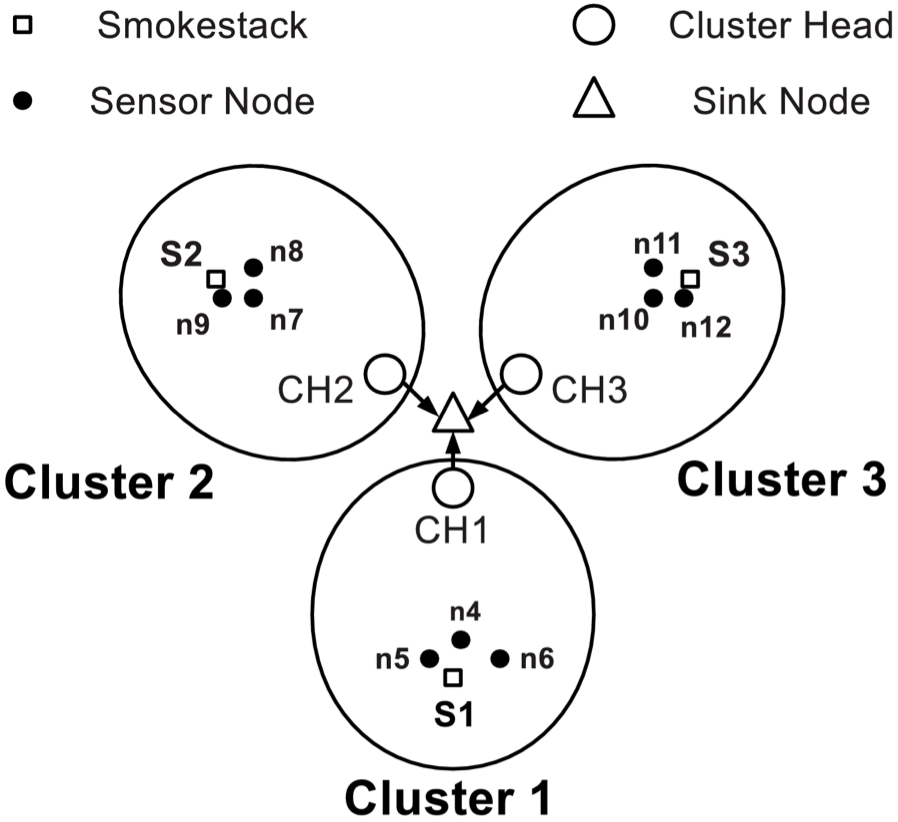
\includegraphics[width=.55\textwidth]{images/raster/scenario}
\caption{Chimney scenario}
\label{fig:chimney-scenario}
\end{figure} 
%
It consists of an industrial area in which three independent plants release pollutant into the air, through smokestack S1, S2 and S2 respectively. In the field there is also a WSN. It monitors pollution levels and detects any plants's abnormal behavior.

The WSN is composed by one sink and three clusters. Each cluster is associated with one smokestack and consists of one \emph{cluster head} and three \emph{sensor nodes}.

Each sensor node periodically senses the pollution in its own cluster and sends reports to its own cluster head. Periodically, each cluster head computes the average pollution level according to the received reports and delivers it to the sink node. Finally, the sink node checks whether any report exceeds a given threshold.

\paragraph{Configurations}
You can see all the possible configurations by following command: \footnote{If you have not exported the environment variable \texttt{~/asfpp/bin} as explained in the section~\ref{sec:asfpp-install}, you have to specify the entire relative path \texttt{../../bin/Castalia}.}
%
\begin{lstlisting}[language={terminal}]
@~/asfpp/Simulations/chimneys-3smokes $@ Castalia 
@
List of available input files and configurations:

* omnetpp.ini
	General
	misread
	misplace
	injection@
\end{lstlisting}

There are 4 different configurations. \texttt{General} is the Castalia's standard configuration, i.e. a configuration without cyber-physical attacks. \texttt{misread}, \texttt{misplace} and \texttt{injection} refer different attacks.

To automate the plotting of simulations's results, it is provided a bash script \texttt{run.sh}.


\subsubsection{General (no attack)}
\label{subsec:no-attack}
The first run refers to the configuration \texttt{General}.  If you are interested in the correctness of data, you can reapeat the simulation for $N$ times, for example 5:
%
\begin{lstlisting}[language={terminal}]
@~/asfpp/Simulations/chimneys-3smokes$@ ./run.sh
@
List of available input files and configurations:

* omnetpp.ini
	General
	misread
	misplace
	injection

Using input file 'omnetpp.ini'
Enter the 'Config' to run:@ General
@Using configuration 'General'
Enter the number of repetitions:@ 5
\end{lstlisting}

The script \texttt{run.sh} moves all the simulative results into a new folder, for example \texttt{General-20151014-172931}. The name of the new folder is that of the configuration that was used to which it is appended a timestamp.

Figure~\ref{fig:no-attack} (stored into the folder \texttt{plot}) shows the results of the simulation just performed.
%
\begin{figure}
\centering
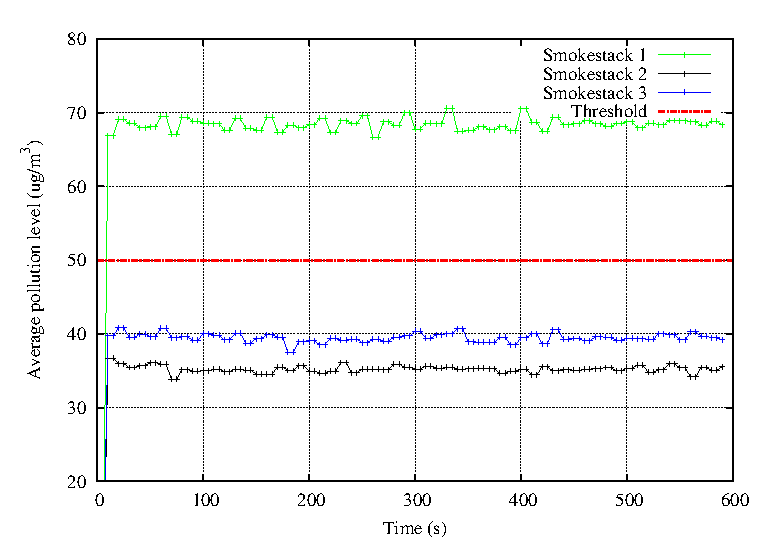
\includegraphics[width=.8\textwidth]{images/raster/general}
\caption{Results of configuration \texttt{General}}
\label{fig:no-attack}
\end{figure} 
%
The threshold (dashed red line) is fixed at 50 $\frac{\mu g}{m^3}$. The graph shows that emissions from S1 are exceeding the threshold.



\subsubsection{misread}
This is a \emph{physical} attack where sensor readings of 4, 5 and 6 tampered with the aim to lowering the value of their measurements.
%
\begin{lstlisting}[language={terminal}]
@~/asfpp/Simulations/chimneys-3smokes$@ ./run.sh
@
List of available input files and configurations:

* omnetpp.ini
	General
	misread
	misplace
	injection

Using input file 'omnetpp.ini'
Enter the 'Config' to run:@ misread
@Using configuration 'General'
Enter the number of repetitions:@ 5
\end{lstlisting}
%
Figure~\ref{fig:misread} shows the results of the simulation just performed.
%
\begin{figure}
\centering
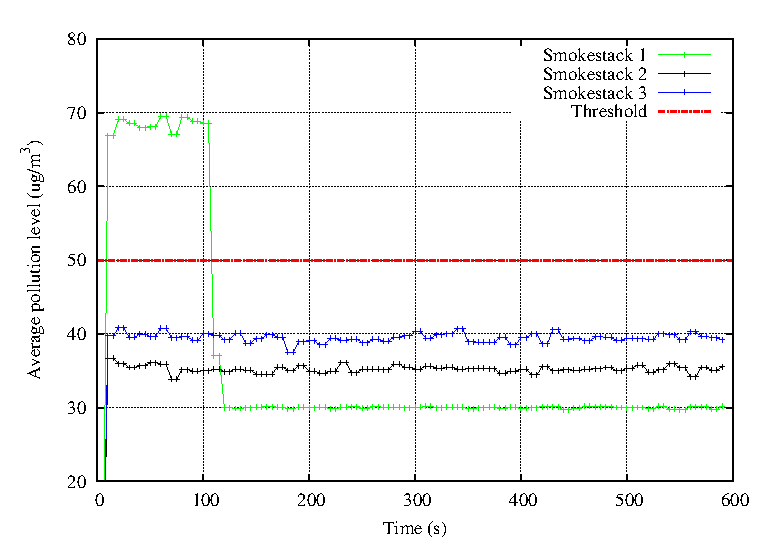
\includegraphics[width=.8\textwidth]{images/raster/misread}
\caption{Results of configuration \texttt{misread}}
\label{fig:misread}
\end{figure} 
%
By performing the attack \texttt{misread}, the emissions from S1 appear to be regular.


\subsubsection{misplace and injection}
You can run other ready-to-use attacks as explained above.



\subsection{Run your own attack}
\label{subsec:run-your-own-attack}
Before running your own attack, you must follow the following steps:
%
\begin{enumerate}
\item edit an \texttt{adl} file by using any text editor;
\item interpret the \texttt{adl} file by using the Attack Description Interpreter (ADI);
\item edit the file \texttt{omnetpp.ini} to include a configuration that refers the new attack.
\end{enumerate}


\paragraph{Write your own \texttt{adl} file}
To write your own attack you must know the Attack Description Language (ADL), see section \ref{sec:adl}. You can write a new attack by editing editing a new \texttt{adl} file. For example, we can create the file \texttt{destroy.asl} that contains the description of an attack that destroys nodes 4, 5 and 6.
%
\begin{lstlisting}[language={adl}]
# destroy attack
destroy(4, 100)
destroy(5, 100)
destroy(6, 100)
\end{lstlisting}

\paragraph{Interpret the \texttt{adl} file}
After creating the file that contains the description of the attack, you have to intepret it by using the ADI. The general sintax to invoke the ADI is the following:
%
\begin{lstlisting}[language={terminal}]
python path/interpreter.py -i <file.adl> -o <file.xml>
\end{lstlisting}
%
The input file is mandatory. You can specify the name of the \texttt{xml} file, that is the output of the ADI. If the file \texttt{destroy.adl} is stored in \texttt{~/asfpp/Simulations/chimneys-3smokes/attacks}, to interpret it type:
%
\begin{lstlisting}[language={terminal}]
@~/asfpp/Simulations/chimneys-3smokes/attacks$@ python ../../../interpreter/interpreter/interpreter.py -i destroy.adl
@Using default output filename 'destroy.xml'@
\end{lstlisting}
%
The output file is \texttt{destroy.xml}.


\paragraph{Edit the file \texttt{omnetpp.ini}}
The last step is to edit the configuration file \texttt{omnetpp.ini}. It is composed of several parts, each of which describes a particular configuration.
The firsts part is always referred to the configuration \texttt{General}, which is mandatory. After the configuration \texttt{General}, you can describe other configurations. 

To describe a new configuration that includes the file \texttt{destroy.xml}, you have to append to the configuration file the following lines:
%
\begin{lstlisting}[language={terminal}]
[Config destroy]
SN.configurationFile = "attacks/destroy.xml"
\end{lstlisting}
%
For a better understanding about the configuration file, see the user manuals of \omnet and Castalia. 

\paragraph{Run the simulation}
Finally you can run the simulation that includes the attack destroy.
% !TEX root = ../asfpp-user-manual.tex

\section{Attack Description Language}
\label{sec:adl}

The Attack Description Language (ADL) is a very simple and flexible high-level language. It provides to users a set to primitives that can be combined to describe cyber-physical attacks.

\subsection{Attacks}
\asf conceives an attack as a ordered sequence of events. Events are described by using the primitives provided by the ADL. Each primitive produces a particular effect. 
Primitives are organized into two sets, as described below.
%
\begin{itemize}
% node primitives
\item [i)] \emph{node primitives}, that account for physical attacks, and allow users to describe alterations in node behavior. In particular, the node primitives are:
\begin{itemize}
\item \texttt{destroy}, destroys a node from the sensor network;
\item \texttt{disable}, disables a node's NIC;
\item \texttt{move}, misplaces a node;
\item \texttt{fakeread}, tampers a node's sensor readings.
\end{itemize}

% message primitives
\item [ii)] \emph{message primitives}, that account for cyber attacks, and allow users to describe actions on network messages. In particular, the message primitives are:
\begin{itemize}
\item \texttt{drop}, discards a certain packet;
\item \texttt{create}, creates from scratch a new packet of a certain type;
\item \texttt{clone}, creates a perfect copy of a given packet;
\item \texttt{retrieve}, inspects a certain field of a given packet;
\item \texttt{change}, changes the content of a particular field of a given packet;
\item \texttt{send}, sends a packet (one created from scratch) to the bottom layer in the communication stack;
\item \texttt{put}, sends a certain packet to a list of recipient nodes.
\end{itemize}
\end{itemize}

The user can combine the primitives to describe complex attacks. By using node primitives, the user can describe \emph{physical attacks}, e.g. destruction of nodes or alteration of sensed values. By using message primitives, the user can describe \emph{cyber attacks}, e.g. dropping, alteration injection or eavesdropping of messages.
In addition to primitives, the ADL provides some support structures to users as filter statements to intercept certain messages, loop statements to build cyclic operations,  lists, variables, expression solver engines, etc.


% node primitives
\subsection{Node primitives}
Node primitives act on the nodes and are used to describe physical attacks.
% destroy
\subsubsection{destroy}
The primitive \texttt{destroy} removes a target node from the simulation field, preventing it from doing any operation.
%
\begin{lstlisting}[language={adl}]
destroy(node_id, occurrence_time)
\end{lstlisting}
%
Parameters:
%
\begin{itemize}
\item[-] \texttt{node\_id} is the id of the target node;
\item[-] \texttt{occurrence\_time} is the time in which the primitive is performed.
\end{itemize}

% disable
\subsubsection{disable}
The primitive \texttt{disable} disables the NIC of a target node, preventing it from taking part in further communications. The node can still continue to perform all the other operations.
%
\begin{lstlisting}[language={adl}]
disable(node_id, occurrence_time)
\end{lstlisting}
%
Parameters:
%
\begin{itemize}
\item[-] \texttt{node\_id} is the id of the target node;
\item[-] \texttt{occurrence\_time} is the time in which the primitive is performed.
\end{itemize}

% move
\subsubsection{move}
The primitive \texttt{move} misplaces a target node.
%
\begin{lstlisting}[language={adl}]
move(node_id, occurrence_time, coord_x, coord_y, coord_z)
\end{lstlisting}
%
Parameters:
%
\begin{itemize}
\item[-] \texttt{node\_id} is the id of the target node;
\item[-] \texttt{occurrence\_time} is the time in which the primitive is performed;
\item[-] \texttt{coord\_x} is the target x coordinate;
\item[-] \texttt{coord\_y} is the target y coordinate;
\item[-] \texttt{coord\_z} is the target z coordinate.
\end{itemize}

% fakeread
\subsubsection{fakeread}
The primitive \texttt{fakeread} tampers the sensor readings of a target node.
%
\begin{lstlisting}[language={adl}]
fakeread(node_id, occurrence_time, sensor_id, function)
\end{lstlisting}
%
Parameters:
%
\begin{itemize}
\item[-] \texttt{node\_id} is the id of the target node;
\item[-] \texttt{occurrence\_time} is the time in which the primitive is performed;
\item[-] \texttt{sensor\_id} is the id of sensor (of the target node);
\item[-] \texttt{function} is the mathematical function used to compute the tampered value.
\end{itemize}



% message primitives
\subsubsection{Message primitives}
Message primitives act on messages and are used to describe cyber attacks.

% drop
\subsubsection{drop}
The primitive \texttt{drop} discards a target packet.
%
\begin{lstlisting}[language={adl}]
drop(pck, threshold)
\end{lstlisting}
%
Parameters:
%
\begin{itemize}
\item[-] \texttt{pck} is the target packet;
\item[-] \texttt{threshold} is the threshold that models the probability of dropping the target packet.
\end{itemize}

% create
\subsubsection{create}
The primitive \texttt{creates} creates a new packet from scratch. The new packet can contain other encapsulated packets. A single invocation makes it possible to specify the types of all the packets, from the outer one to the inner one.
%
\begin{lstlisting}[language={adl}]
create(pck, layer_n, type_n, layer_n-1, type_n-1, ...)
\end{lstlisting}
%
Parameters:
%
\begin{itemize}
\item[-] \texttt{pck} is the new packet;
\item[-] \texttt{layer\_n, type\_n} is the couple that defines the type of the outer packet that belongs to the layer n;
\item[-] \texttt{layer\_n-1, type\_n-1} is the couple that defines the type of the inner packet that belongs to the layer n-1.
\end{itemize}

% clone
\subsubsection{clone}
The primitive \texttt{clone} clones a target packet, i.e. it creates a perfect copy of the target packet.
%
\begin{lstlisting}[language={adl}]
clone(src_pkt, dst_pck)
\end{lstlisting}
%
Parameters:
%
\begin{itemize}
\item[-] \texttt{src\_pck} is the source packet (i.e. the packet to clone);
\item[-] \texttt{dst\_pck} is the destination packet (i.e. the cloned one).
\end{itemize}

% retrieve
\subsubsection{retrieve}
The primitive \texttt{retrieve} copies the value of a target field (of a target packet) into a variable.
%
\begin{lstlisting}[language={adl}]
retrieve(pck, field_name, variable_name)
\end{lstlisting}
%
Parameters:
%
\begin{itemize}
\item[-] \texttt{pck} is the packet to inspect;
\item[-] \texttt{field\_name} is the name of the target field;
\item[-] \texttt{variable\_name} is the name of the variable in which to store the retrieved value.
\end{itemize}

% change
\subsubsection{change}
The primitive \texttt{change} changes the value of a target field (of a target packet).
%
\begin{lstlisting}[language={adl}]
change(pck, field_name, variable_name)
\end{lstlisting}
%
Parameters:
%
\begin{itemize}
\item[-] \texttt{pck} is the target packet;
\item[-] \texttt{field\_name} is the name of the target field;
\item[-] \texttt{variable\_name} is the name of the variable which stores the new value.
\end{itemize}

% send
\subsubsection{send}
The primitive \texttt{send} sends a packet that was created from scratch to the next layer in the communication stack . It must be used with packet created by usign the actions \texttt{create} or \texttt{clone}.
%
\begin{lstlisting}[language={adl}]
send(pck, delay)
\end{lstlisting}
%
Parameters:
%
\begin{itemize}
\item[-] \texttt{pck} is the packet to send;
\item[-] \texttt{delay} is the forwarding delay.
\end{itemize}

% put
\subsubsection{put}
The primitive \texttt{put} puts a certain packet in the RX or TX buffer of a set of nodes.
%
\begin{lstlisting}[language={adl}]
put(pck, dst_nodes, TX|RX, TRUE|FALSE, delay)
\end{lstlisting}
%
Parameters:
%
\begin{itemize}
\item[-] \texttt{pck} is the packet to put;
\item[-] \texttt{dst\_nodes} is the list of nodes;
\item[-] \texttt{TX|RX} defines in which buffer to put the packet (in the TX buffer or in the RX buffer);
\item[-] \texttt{TRUE|FALSE} defines in use or not the wireless channel as communication channel;
\item[-] \texttt{delay} is the forwarding delay.
\end{itemize}














\subsection{Support structures}
The ADL provides a set of support structures to allow the user to describe even complex attacks.

% variables, packets and lists
\subsubsection{Variables, lists and packets}

% variables
\paragraph{Variables}
The ADL is dynamically typed. It provides the keyword \texttt{var} to declare and initialize variables.
%
\begin{lstlisting}[language={adl}]
var foo
\end{lstlisting}
%
Variables must be declared before use.

If a variable is declared and initialized inside a loop statement, the initialization is carried out only in the first iteration.
%
\begin{lstlisting}[language={adl}]
<loop_statement_begin>
var foo = 0
...
foo += 1
<loop_statement_end>
\end{lstlisting}
%
Tha var foo is initialized to 1. At the end of the 1st iteration its value is 1, at the end of the 2nd iteration its value is 2, at the end of the 3rd iteration its value is 3, and so on.

% lists
\paragraph{Lists}
The ADL provides the keyword \texttt{list} to declare lists of values.
%
\begin{lstlisting}[language={adl}]
list nodes_list = {1, 2, 3, 4, 5}
\end{lstlisting}
%
Lists must be declared before use.

% packets
\paragraph{Packets}
The ADL provides the keyword \texttt{packet} to declare a reference to packets.
%
\begin{lstlisting}[language={adl}]
packet my_pck
\end{lstlisting}

% functions
\subsubsection{Functions}
The ADL provides the keyword \texttt{function} to declare mathematical functions to be evaluated by nodes at runtime. The user can use 2 independent variables:
%
\begin{itemize}
\item[-] \texttt{t} is the simulation time, evaluated at runtime;
\item[-] \texttt{s} is the sensor reading value, evaluated at run time. 
\end{itemize}
%
At the moment, functions can be used only if combined with the primitive \texttt{fakeread}.
%
\begin{lstlisting}[language={adl}]
function f1 =  "sin(2*pi*t) + 0.75*s"
fakeread(1, 100, 0, f1)
\end{lstlisting}
%
The independet variable \texttt{s} refers the sensor reading value of the sensor 0 of the node 1.


% expressions
\subsubsection{Expressions}
An expression is an ordered collection of operands, namely numbers, strings or variables, and operators. Figure~\ref{tab:expression-table} shows the ADL expression table.
%
\begin{lstlisting}[language={adl}]
var result
var operand1 =  2
var operand2 =  7
result = operand1 +  operand2
result = "Hello"  # legal expression
result += ", world!"  # legal expression
var operand3 =  5
result += operand3  # illegal expression
\end{lstlisting}
%
% ADL expression table
\begin{table}
\centering
\subfloat[Assignment operators]{
\begin{tabular}{ccc}
\toprule
\textbf{operator}&\textbf{numbers}&\textbf{strings}\\
\midrule
$=$			& supported		& supported		\\
$+=$			& supported		& not supported	\\
$-=$			& supported		& not supported	\\
$\times =$		& supported		& not supported	\\
$/=$			& supported		& not supported	\\
$\div =$		& supported		& not supported	\\
\bottomrule
\end{tabular}
}\\
\subfloat[Arithmetic operators]{
\begin{tabular}{ccc}
\toprule
\textbf{operator}&\textbf{numbers}&\textbf{strings}\\
\midrule
$+$		& supported		& supported		\\
$-$		& supported		& not supported	\\
$\times$	& supported		& not supported	\\
$/$		& supported		& not supported	\\
$\div$	& supported		& not supported	\\
\bottomrule
\end{tabular}
}\\
\subfloat[Comparison operators]{
\begin{tabular}{ccc}
\toprule
\textbf{operator}&\textbf{numbers}&\textbf{strings}\\
\midrule
$<$		& supported		& supported	\\
$>$		& supported		& supported	\\
$<=$		& supported		& supported	\\
$>=$		& supported		& supported	\\
$==$		& supported		& supported	\\
$!=$		& supported		& supported	\\
\bottomrule
\end{tabular}
}\\
\subfloat[Logical operators]{
\begin{tabular}{ccc}
\toprule
\textbf{operator}&\textbf{numbers}&\textbf{strings}\\
\midrule
AND		& supported		& supported	\\
OR		& supported		& supported	\\
\bottomrule
\end{tabular}
}
\caption{ADL expression table}
\label{tab:expression-table}
\end{table}

% loop statements
\subsubsection{Loop statements}
The ADL provides a \emph{loop statement} that allows the user to specify the occurrence of a list of events described through message primitives. Events occurrence may depend or not on the evaluation of a conditional statement. It is possible to use two types of loop statemens:
%
\begin{itemize}
\item [i)] \emph{conditional loop statement}, if the execution of the message primitives contained in the loop statement depends on the evaluation of a conditional statements;
\item [ii)] \emph{unconditional loop statement}, if the message primitives contained in the loop statement are executed unconditionally.
\end{itemize}

% conditional
\paragraph{Conditional loop statement}
A conditional loop statement has the structure that follows.
%
\begin{lstlisting}[language={adl}]
from T nodes in <nodes_list> do { 
<packet_filter>
    <List of message primitives>
}
\end{lstlisting}
%
The execution of the message primitives contained inside a conditional loop statement depends on the evaluation of a \emph{packet filter}. 

\paragraph{Packet filter}
The packet filter is a set of simple boolean conditions c1, c2, ..., cN joined by logic operators, i.e. AND, OR, and NOT. 
Each condition is related to a certain field of a certain type of packet. Accordingly, the packet filter is evaluated by nodes at runtime.
Nodes inspect packets flowing through their communication stack. If a packet matches the packet filter, the message primitives contained in the conditional loop statements are executed. 

The ADL provides the keyword \texttt{filter} to describe the packet filter.
%
\begin{lstlisting}[language={adl}]
filter (layer5.source == 10 AND layer4.sourcePort == 1000)
\end{lstlisting}
%
In the example above, all packets belonging (at least) to the layer 4 of the TCP/IP stack having the field \texttt{source} in the layer 5 setted to 10 and the field \texttt{sourcePort} of the layer 4 setted to 1000 match the packet filter.
The \asf provides the keyword \texttt{original} to refer the original packet intercepted by the packet filter.

What follows is an example of conditional loop statement. Starting from time 200 s, nodes 1, 2, and 7 intercept all packets travelling through their communication stack having the the field \texttt{sourcePort} of layer 4 setted to 1000. Then, such nodes check if each intercepted packet satisfies the packet filter. In case of a positive match, the message primitives contained in the conditional loop statements are executed.
%
\begin{lstlisting}[language={adl}]
list nodes_list = {1, 2, 7}
...
from 200 nodes in nodes_list do {
filter(layer4.sourcePort == 1000)
    <List of message primitives>
}
\end{lstlisting}

Note that the execution frequency of the conditional loop statements can't be setted by the user but it depends on the dynamic of the simulation (i.e. the frequency with which packets are generated) and on the evaluation at runtime of the packet filter.

% unconditional
\subsubsection{Unconditional loop statements}
Unlike conditional loop statements, the unconditional are not related to interception of packets by network nodes. However, new packets can be created, and possibly cloned, in order to be naughtly injected into the network. The user must specify the time \texttt{T} starting from which the attack takes place, and the occurrence period \texttt{P} according to which the attack has to be repeatedly reproduced over time. 

The unconditional loop statements concern the network nodes but do not run directly from them. \asf provides a particular node, namely the Global Filter, which is not part of the network and has the task to execute the attacks based on the unconditional loop statements.

An unconditional loop statement has the structure that follows.
%
\begin{lstlisting}[language={adl}]
from T every P do { 
    <List of message primitives>
}
\end{lstlisting}
%
What follows is an example of unconditional loop statement. Starting from time 200 s, every 0.1 s (10 Hz), the Global Filter executes the list of message primitives.
%
\begin{lstlisting}[language={adl}]
from 200 every 0.1 do {
    <List of message primitives>
}
\end{lstlisting}

Note that the user can set the execution frequency (even to 0 to obtain a one-time execution) of the unconditional loop statements.



% attack types
\subsection{Attack types}
\label{ss:attacktypes}
By using the primitives and the support structures provided by the ADL (in particular the loop statements), the user can describe three different types of attacks:
%
\begin{itemize}
\item [i)] \emph{physical attacks}, that consist of a single node primitive;
\item [ii)] \emph{conditional attacks}, that consist of a set of message primitives contained in conditional loop statements;
\item [iii)] \emph{unconditional attacks}, that consis of a set of message primitives contained in unconditional loop statements.
\end{itemize}
%
Physical and conditional attacks are performed directly by nodes, unconditional ones instead are performed by a particular node provided by \asf which does is not part of the network.

% physical attacks
\subsubsection{Physical attacks}
A physical attack consists of a single node primitive and is triggered directly by the node indicated in the primitive.
%
\begin{lstlisting}[language={adl}]
destroy(1, 150)
\end{lstlisting}
%
In the example above, the node 1 is destroyed at time 150. In particular, it is the node itself that triggers its own destruction.

% conditional attacks
\subsubsection{Conditional attacks}
A conditional attack consists of a set of message primitives contained in a conditional loop statement. Conditional attacks are performed directly by nodes specified in the conditional loop statement. As specified above, a node performs the primitives contained in the loop statement only if the current packet matches the packet filter.
%
\begin{lstlisting}[language={adl}]
list nodes_list = {1, 3, 7}
...
from 150 nodes in nodes_list do {
filter (layer4.sourcePort == 1000)    
    var sourcePort = 1500
    change(original, layer4.sourcePort, sourcePort)
}
\end{lstlisting}
%
In the example above, from time 150, nodes 1, 3 and 7 change the value of the field \texttt{sourcePort} of the layer 4 from 1000 to 1500, only if the current packet matches the packet filter. The current packet for nodes 1, 3 and 7, i.e. the packet passing through the communication stack of nodes 1, 3 and 7 respectively, matches the packet filter if the value of the field \texttt{sourcePort} of the layer 4 is 1000. 
The keyword \texttt{original} refers the original packet intercepted by the packet filter.

% unconditional attakcs
\subsubsection{Unconditional attacks}
An unconditional attack consists of a set of message primitives contained in an unconditional loop statement. Unconditional attacks are not performed directly by nodes but are executed by the Global Filter, a particular node provided by \asf which is not part ot the newtork.
%
\begin{lstlisting}[language={adl}]
list nodes_list = {1, 3, 7}
...
from 150 every 0.1 do{
    # declare a packet
    packet my_packet
    # declare and initialize variables
    var sensorId = 0
    var value = 50
    var seqNumb = 1000
    # create a new packet from scratch
    create(my_packet, layer5, 0001)
    # set values in the packet fields 
    change(my_packet, layer5.sensorId, sensorId)
    change(my_packet, layer5.seqNumb, seqNumb)
    change(my_packet, layer5.value, value)
    # put the new packet into the RX buffer of nodes 1,3,7, without forwarding delay
    put(my_packet, nodes_list, RX, 0)
    # update seqNumb
    seqNumb += 1
}
\end{lstlisting}
%
In the example above, from time 150, the Global Filter creates a new packet, sets its fields appropriately and puts the packet in the RX buffer of nodes 1, 3 and 7.

% expected knowledge
\subsubsection{Expected knowledge}
In general, to evaluate the effects of fairly simple attacks, \asf requires to the user only the knowledge about the network topology.
Instead, to perform more complex attacks that involves the creation of packets and the alteration of their fields (even the creation of protocols's signaling messages), \asf requires to the user the knowledge of the:
%
\begin{itemize}
\item[-] communication stack (encapsulation/decapsulation mechanisms);
\item[-] structure of packets (headers and payload);
\item[-] protocols running on each layer.
\end{itemize}
%
However, given that the majority of attacks (except those special ones) does not require any in-depth knowledge, \asf is a very user friendly tool.


\subsection{Attack description}
\label{ss:attackdefinition}


\subsubsection{ADI output}
The following examples show how the Attack Description Interpreter interprets physical, conditional and unconditional attacks.

% interpreted physical attack
\paragraph{Interpreted physical attack}
The listing below describes a physical attack in which the readings of the sensor 0 of the node 2 are tampered from time 150 by using the function f1.
%
\begin{lstlisting}[language={adl}]
function f1 = "sin(2*pi*t) + 0.75*s"
fakeread(2, 150, 0, f1)
\end{lstlisting}
%
The physical attack above is interpreted by the ADI as follows:
%
\begin{lstlisting}[language={xml}]
<configuration>
    <Physical>
        <Attack>
            <start_time>150</start_time>
            <node>2</node>
            <action>
                <name>Fakeread</name>
                <parameters>sensor_id:0:function:sin(2*pi*t) + 0.75*s</parameters>
            </action>
        </Attack>
    </Physical>
</configuration>
\end{lstlisting}


% interpreted conditional attack
\paragraph{Interpreted conditional attack}
The listing below describes a conditional attack in which, from time 150, nodes 1, 3 and 7 change the value of the field \texttt{sourcePort} of the layer 4 from 1000 to 1500, only if the current packet matches the packet filter.
%
\begin{lstlisting}[language={adl}]
list nodes_list = {1, 3, 7}
from 150 nodes in nodes_list do {
filter (layer4.sourcePort == 1000)    
    var sourcePort = 1500
    change(original, layer4.sourcePort, sourcePort)
}
\end{lstlisting}
%
The conditional attack above is interpreted by the ADI as follows:
%
\begin{lstlisting}[language={xml}]
<configuration>
    <Conditional>
        <Attack>
            <start_time>150</start_time>
            <node>1:3:7</node>
            <var><name>sourcePort</name><value>1500</value><type>NUMBER</type></var>
            <filter>[:layer4.sourcePort:==:1000:]</filter>
            <action>
                <name>Change</name>
                <parameters>packetName:original:field_name:layer4.sourcePort:value:sourcePort</parameters>
            </action>
        </Attack>
    </Conditional>
</configuration>
\end{lstlisting}


% interpreted unconditional attack
\paragraph{Interpreted unconditional attack}
The listing below describes an unconditional attack in which, from time 150, the Global Filter creates a new packet, sets its fields appropriately and puts the packet in the RX buffer of nodes 1, 3 and 7.
%
\begin{lstlisting}[language={adl}]
list nodes_list = {1, 3, 7}
from 150 every 0.1 do{
    # declare a packet
    packet my_packet
    # declare and initialize variables
    var sensorId = 0
    var value = 50
    var seqNumb = 1000
    # create a new packet from scratch
    create(my_packet, layer5, 0001)
    # set values in the packet fields 
    change(my_packet, layer5.sensorId, sensorId)
    change(my_packet, layer5.seqNumb, seqNumb)
    change(my_packet, layer5.value, value)
    # put the new packet into the RX buffer of nodes 1,3,7, without forwarding delay
    put(my_packet, nodes_list, RX, 0)
    # update seqNumb
    seqNumb += 1
}
\end{lstlisting}
%
The conditional attack above is interpreted by the ADI as follows:
%
\begin{lstlisting}[language={xml}]
<configuration>
    <Unconditional>
        <Attack>
            <start_time>150</start_time>
            <frequency>0.1</frequency>
            <var><name>seqNumb</name><value>1000</value><type>NUMBER</type></var>
            <var><name>sensorId</name><value>0</value><type>NUMBER</type></var>
            <var><name>1</name><value>1</value><type>NUMBER</type></var>
            <var><name>value</name><value>50</value><type>NUMBER</type></var>
            <action>
                <name>Create</name>
                <parameters>packetName:my_packet:layer5..type:1</parameters>
            </action>
            <action>
                <name>Change</name>
                <parameters>packetName:my_packet:field_name:layer5.sensorId:value:sensorId</parameters>
            </action>
            <action>
                <name>Change</name>
                <parameters>packetName:my_packet:field_name:layer5.seqNumb:value:seqNumb</parameters>
            </action>
            <action>
                <name>Change</name>
                <parameters>packetName:my_packet:field_name:layer5..value:value:value</parameters>
            </action>
            <action>
                <name>Put</name>
                <parameters>packetName:my_packet:nodes:1|3|7:direction:RX:false:delay:0</parameters>
            </action>
            <action>
                <name>Expression</name>
                <item>1</item>
                <item>+=</item>
                <item>seqNumb</item>
            </action>
        </Attack>
    </Unconditional>
</configuration>
\end{lstlisting}

Note that expressions are handled by \asf as additional events.
\printindex

\end{document}
